\documentclass[abstract=on,9pt,twocolumn]{scrartcl}

\usepackage{ucs}
\usepackage[utf8x]{inputenc}
\usepackage[T1]{fontenc}
\usepackage[english]{babel}

%\usepackage{graphics}%	images other than eps

\usepackage[paper=a4paper,top=2cm,left=1.5cm,right=1.5cm,bottom=2cm,foot=1cm]{geometry}

\usepackage{relsize}%	relative font sizes

\usepackage[retainorgcmds]{IEEEtrantools}%	IEEEeqnarray
\setlength{\IEEEnormaljot}{4\IEEEnormaljot}

\usepackage{graphicx}
\usepackage{epstopdf}
\usepackage{indentfirst}
\usepackage{hyperref}
%\usepackage{cleveref}
\usepackage[noabbrev]{cleveref}
\usepackage{listings}
\usepackage{color}

%%%%%%%%%%%%%%%%
%  title page  %
%%%%%%%%%%%%%%%%
\titlehead{University of Minho \hfill Master's Degree in Informatics Engineering\\	Department of Informatics \hfill Parallel and Distributed Computing}

\title{A finite volume case study from an industrial application}

\subtitle{OpenMP: analysis and improvements}

\author{{\larger Group 1}\\Miguel Palhas \hfill--- \texttt{\smaller pg19808@alunos.uminho.pt}\\Pedro Costa \hfill--- \texttt{\smaller pg19830@alunos.uminho.pt}\\\smaller Stéphan Clain (co-Advisor)\\
}

\date{Braga, April 2012}

\subject{Integrated Project}


%%%%%%%%%%%
%  Hacks  %
%%%%%%%%%%%

%	Paragraph (title) with linebreak
\newcommand{\paragraphh}[1]{\paragraph{#1\hfill}\hfill

}

%	Add "Appendix" to the appendices titles, but not to the references
\usepackage{ifthen}
\newcommand*{\appendixmore}{%
  \renewcommand*{\othersectionlevelsformat}[1]{%
    \ifthenelse{\equal{##1}{section}}{\appendixname~}{}%
    \csname the##1\endcsname\autodot\enskip}
  \renewcommand*{\sectionmarkformat}{%
    \appendixname~\thesection\autodot\enskip}
}




\begin{document}
\maketitle

\begin{abstract}
Due to a lack of scalability in previous approaches, the latest version of a scientific application meant to simulate the spread of a pollutant in a given environment was analyzed and measured.

The results showed poor locality caused by AOS data structures, unfit for the problem.

A new version was implemented using SOA data structures which presented higher speedups, both when compared with the original code or due to the addition of thread-level parallelism.
\end{abstract}

\section{Introduction}
% why are we doing this report
This document follows a previous report where the \texttt{polu} application -- which computes the evolution of a pollutant in a given environment -- was studied in order to find possibilities of optimization and/or parallelization.

The \texttt{polu} application works like a heartbeat algorithm with no communication (since it is executed in a single computation node). The algorithm used by the program sees the environment as a discrete mesh (represented by its cells and edges) and loops until the specified time interval is reached. At each iteration of this main loop, the flux of pollution is calculated in each edge (first phase of the algorithm, performed by a function named \texttt{compute\_flux}), which is followed by the update of the mesh pollution levels in each cell (second and last phase of the algorithm, performed by the \texttt{update} function).

Several changes were performed in the original \texttt{polu} code in order to allow parallelization and/or improve performance. The most important of these optimizations involved changing the data structures (originally implemented as \textit{Arrays-of-Pointers}) to \textit{Arrays-of-Structures}. This change removed the excessive dereferencing caused by deep chains of pointers in the original structures, which effectively reduced data access time improved locality.

Despite the many optimizations added, the implementation of a parallel version using OpenMP directives achieved speedup values which were much lower than expected.

The goal of this stage is to study the reasons behind the lack of scalability in the code of the previous report and present an improved version based on that information. A detailed profiling is performed on both versions to evaluate the improvement's extent and identify performance limitations.

This document begins with a deep analysis of the previous implemented code in \cref{sec:aos}, meant to find the problems behind the lack of scalability presented in the last report. \Cref{sec:soa} presents an improved version of the \texttt{polu} program, guided by the information retrieved before. The discussion of results in this section includes a direct comparison between the two versions. The final conclusions are presented in \cref{sec:conclusion}. Due to the need to keep this document's structure in such a way that it is able to reflect the temporal evolution of the project, the environmental setup is described in \cref{sec:environment}, followed by the methodology in \cref{sec:method}. Additionally, a description of the hardware events used with the PAPI library may be found in \cref{sec:events}, and an explanation on how the rooflines in this document were built may be found in \cref{sec:roofline}.









\section{Analysis}
\label{sec:aos}
% why weren't the goals achieved in the last report
This section discusses the code implemented for the previous report, analyzing it in an attempt to explain why does it not scale properly.

Lack of scalability can be traced to a number of factors. CPU-bound algorithms tend to be limited by the fraction of parallelizable code -- Amdahl and Gustafson's laws. Memory bound  algorithms are limited by the bandwidth of memory accesses, or by the lack of locality which will prevent the algorithm from using all the available bandwidth.

Locality problems may arise from a variety of issues. This document focus in:
\begin{description}
\item[Structures]{Different structure layouts translate in different memory access patterns.}%Structures with many pointers -- known as \textit{Arrays-of-Pointers (AOP)} -- require higher amounts of dereferencing when accessing memory. \textit{Arrays-of-Structures (AOS)} or  \textit{Structures-of-Arrays (SOA)} are better approaches which do not rely on dereferencing, consequently allowing lower memory access time and better locality. For any given algorithm, one of these two approaches usually improves at least one kind of locality over the other approach.}
\item[Granularity]{When the tasks to be parallelized are too short or small, the overhead of introducing parallelism may exceed the speedup obtained.}% These cases may be solved by increasing the granularity of the tasks (joining several parallel tasks in a single one), which would decrease the frequency of setting up tasks to be run in parallel, and by using static scheduling, which in turn would reduce task creation overhead.}
\item[Synchronization]{Excessive synchronization introduces waiting periods which will increase execution time by preventing the parallel tasks to proceed past a certain point.}% While some algorithms rely on synchronization to assure the correctness of the results (critical zones, barriers, atomic operations), sometimes it is possible to remove, completely or at least partially, the synchronization primitives, thus allowing parallel tasks to be completed with minimum waiting periods.}
\item[Load Balance]{Odd load distribution means a given proceshave more work than others.}% This implies that a given processor may finish its assigned tasks and remain idle while another one is operating to its maximum capacity, possibly with other tasks pending. It is directly related with scheduling.}
\end{description}

The \texttt{polu} algorithm presents both types of locality -- spatial and temporal. Spatial locality -- if a given data element is needed, it is highly probable that adjacent data elements will also be needed -- is found in both core functions, since \texttt{compute\_flux} orderly iterates over every edge, and \texttt{update} orderly iterates over every cell. Temporal locality -- if a given data element is needed, it is highly probable that it will be needed again in the near future -- is also present in both functions, as \texttt{compute\_flux} requires the pollution levels of the cells each edge belong to, and \texttt{update} requires the computed flux of each cell's edges.

Yet, as was explained, both functions possess the two kinds of locality in different data collections. This means they both access edge and cell related data over its course of action, but only one collection will be accessed orderly in each function. This makes it extremely difficult to achieve the locality suited for parallel computation.

The original code implemented data structures as \textit{Arrays-of-Pointers}. In the previous report, the code was modified to remove dereferencing by implementing \textit{Arrays-of-Structures}. Given the facts that each core function accesses data from both edges and cells, and that these functions do not require the same data, the hypothesis remains whether \textit{Structs-of-Arrays} will be a better access pattern, as it would not require the cache to be populated with values which are not necessary to the executing function.

Granularity problems can be measured by comparing the execution time of the parallel tasks with the overhead of creating these tasks. The overhead of using the OpenMP primitives can be obtained using the EPCC OpenMP Microbenchmarks\footnote{Current version is 2.0 -- \url{http://www2.epcc.ed.ac.uk/computing/research_activities/openmpbench/openmp_index.html}}. The execution time of the parallel tasks falls under the first kind of measurements described in \cref{sec:method}.

This algorithm does not present problems related with excessive synchronization or workload imbalance. Regarding synchronization, it exists only between the two phases of the heartbeat, therefore it cannot be removed without compromising the correctness of the algorithm. As for workload balance, each core function performs the same task for each object of the collection it iterates over, resulting in the same computations being performed by each thread.



\subsection{Results \& Discussion}
\label{sec:aos:results}
\Cref{fig:steptimeAOS} shows the execution time for each of the core functions in each type of computational nodes. Regarding parallelism granularity, comparing these execution times with the overheads measured by the EPCC synchronization micro benchmark (see \cref{tab:overhead}) one can easily conclude that it does not represent an issue in the previous implementation. Even in the SeARCH Group 601, where the core functions are able to execute faster, the execution time (around 17 milliseconds for the fastest execution of \texttt{compute\_flux}) greatly exceeds the overhead values (4.79 microseconds in the same nodes).

\begin{table}[!htp]
	\begin{center}
		\begin{tabular}{|c|l|r|}
		\hline
		SeARCH Group & OpenMP Primitive & Overhead ($\mu$s)	\\
		\hline
		201 & \texttt{PARALLEL FOR} & 2.84	\\
		601 & \texttt{PARALLEL FOR} & 4.79	\\
		\hline
		\end{tabular}
	\end{center}
	\caption{Overhead values for the OpenMP primitives used in the parallel versions of the algorithm. Measured using the synchronization EPCC OpenMP Microbenchmark.}
	\label{tab:overhead}
\end{table}

\begin{figure}[!p]
	\begin{center}
		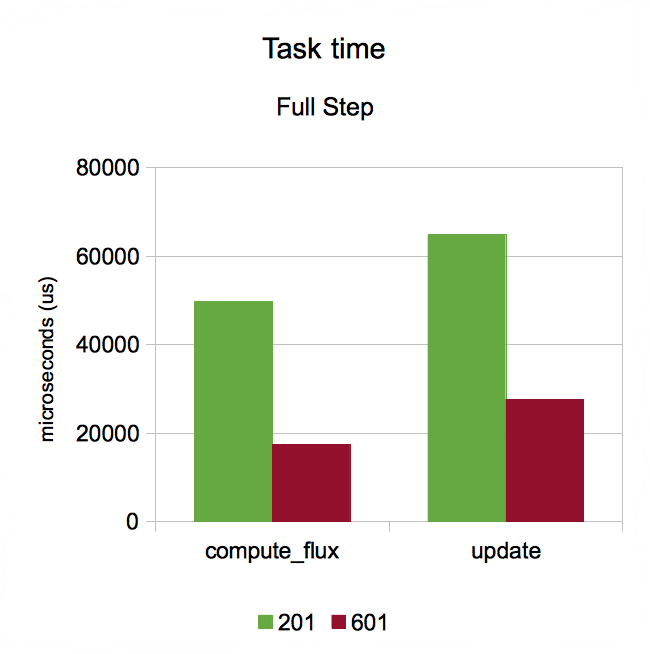
\includegraphics[width=\columnwidth]{images/report.april/steptimeAOS.png}
	\end{center}
	\caption{Median execution times for a full execution of each core function in each kind of computational node. Measured for the previous version (AOS).}
	\label{fig:steptimeAOS}
\end{figure}

\begin{figure}[!p]
	\begin{center}
		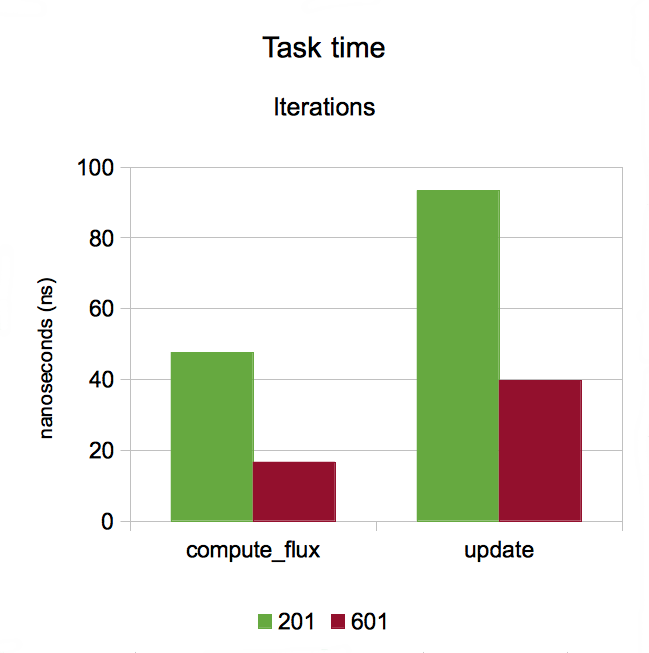
\includegraphics[width=\columnwidth]{images/report.april/tasktimeAOS.png}
	\end{center}
	\caption{Minimum execution times for a single iteration of the inner cycle of each core function in each kind of computational node. Measured for the previous version (AOS).}
	\label{fig:tasktimeAOS}
\end{figure}

As for workload balance, \cref{fig:tasktimeAOS} shows a clear difference between each phase of the algorithm in terms of execution time for a single iteration. Yet, as stated before, this workload does not change in the same function for each thread. In conclusion, the program is heterogeneous (as \texttt{update} takes significantly more to execute than \texttt{compute\_flux}) but each function is homogenous.

\begin{figure}[!p]
	\begin{center}
		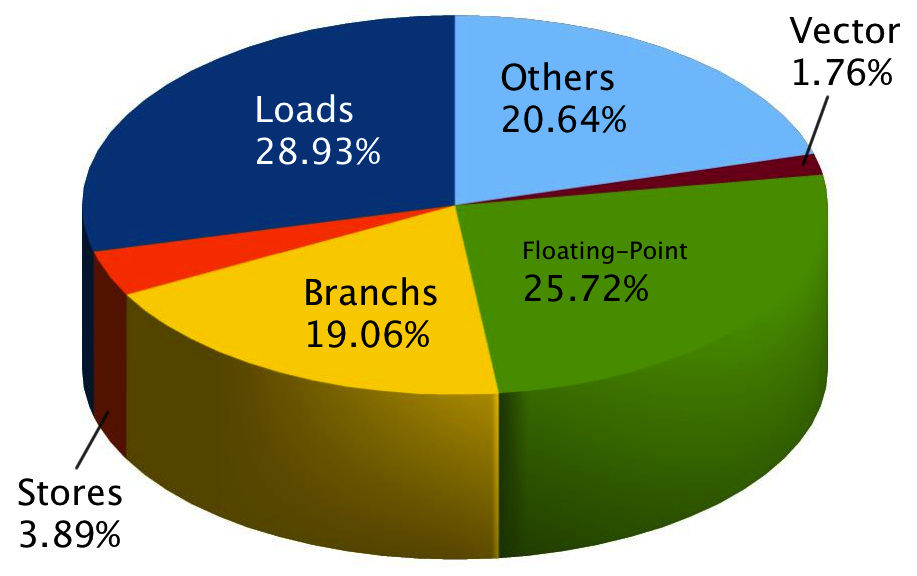
\includegraphics[width=\columnwidth]{images/report.april/instmxAOS.png}
	\end{center}
	\caption{Instruction mix for the previous version (AOS).}
	\label{fig:instmxAOS}
\end{figure}

At this point remains only the memory access pattern as a possible problem in the previous version, which does not present the necessary locality. \Cref{fig:instmxAOS} shows the measured instruction mix for this version, which reveals a broader mix than what was originally considered. The profiling in the previous report was limited to floating-point operations, which are now known to be only a quarter of the completed instructions. This value is exceeded by the fraction of load instructions (almost 30\%), which shows the need the program has to keep data flowing from the memory. The new version must focus in improving locality to reduce the need for RAM accesses.

\begin{figure}[!p]
	\begin{center}
		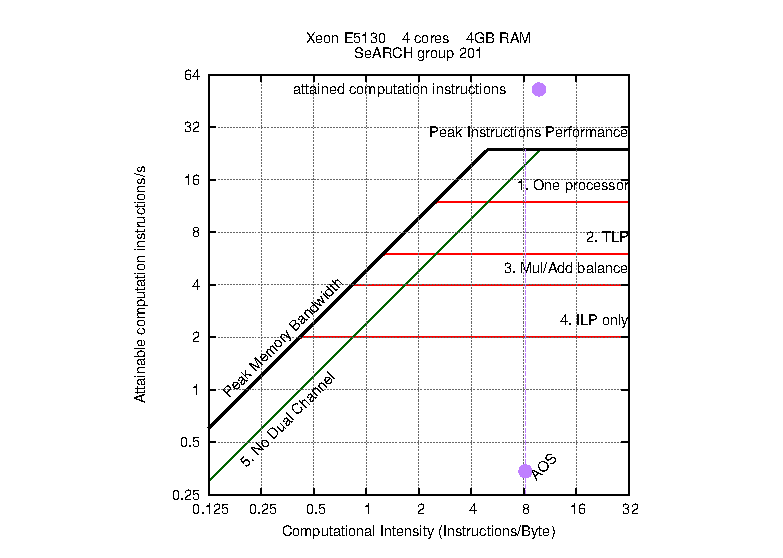
\includegraphics[width=\columnwidth]{images/report.april/rooflineAOS.eps}
	\end{center}
	\caption{Roofline for SeARCH Group 201. The vertical purple line shows the computational intensity of the AOS version, and the point marks the achieved ratio between completed computational instructions and bytes accessed in RAM.}
	\label{fig:rooflineAOS}
\end{figure}

Additionally, since the fraction of floating-point instructions is almost the same as for branches and others\footnote{This number is calculated by subtracting the  measured value of every hardware counter related to instructions from the total of instructions completed. Integer instructions, for example, have no hardware counter available in the used node, and therefore fall in this value.}, computational intensity (ratio between computational instructions and bytes accessed in RAM) is a more complete measure to evaluate the overall algorithm performance\footnote{See \cref{sec:method} for further details.}. \Cref{fig:rooflineAOS} shows the roofline model for the SeARCH Group 201 nodes, with the computational intensity of this version and attained instructions per second -- the program achieves a computational intensity around 8 instructions per accessed byte and attains 0.34 instructions per second.





\section{Improvements}
\label{sec:soa}
% what improvements were performed
Locality optimization in meshes is a deeply researched topic. Yet, the \texttt{polu} algorithm is not a common case. Usually meshes are seen as graphs, and locality is usually optimized for either node or edge access. In the field of computer graphics, research has also been made towards optimizing the access to meshes seen as groups of polygons (or cells). Yet, the core functions of this program iterate over the mesh in different ways, both dealing with cells and edges in different ways. Only \cite{hoppe99} seems focused in improving locality in a useful way for the \texttt{polu} algorithm (by transforming the mesh into an optimized strip of triangles), but the complexity behind Hoppe's work does not fit the time constraints for this project, neither does it guarantee better results.

Instead of using a highly optimized and complex approach to meshes, the option remains to change the data structures from AOS to SOA. As explained before, the new memory access pattern (SOA) would allow each function to exclude any non-useful information, unlike the previous one (AOS) which loads the entire structure for a cell or edge, despite existing pieces of data which are only required for one of the core functions. Additionally, this new approach would favor ordered accesses, since the cache lines would be filled with the same data piece from contiguous cells or edges. These atomic pieces of data are more easily aligned with the limits of a cache line than a structure, reducing the need to replace a cache line in an ordered access to the bare essential.

Since changing the data structures to SOA does not present such a high complexity as Hoppe's work, and since it is trivial how it will improve the algorithm, this was the improvement chosen. The core functions were changed to accept multiple independent arrays of simple data types, instead of a single array with structures holding all the data related to the cells or edges.



\subsection{Results, Discussion and Comparison}

\begin{figure}[!htp]
	\begin{center}
		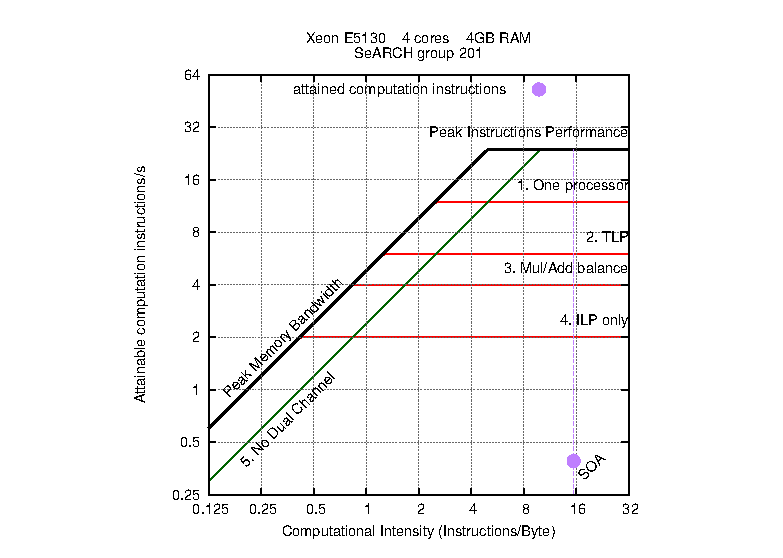
\includegraphics[width=\columnwidth]{images/report.april/rooflineSOA.eps}
	\end{center}
	\caption{Roofline for SeARCH Group 201. The vertical purple line shows the computational intensity of the SOA version, and the point marks the achieved ratio between completed computational instructions and bytes accessed in RAM.}
	\label{fig:rooflineSOA}
\end{figure}

For the roofline (see \cref{fig:rooflineSOA}), the computational intensity is higher (double), but the achieved number of instructions per second remains in a very low value. The question arises: why does this happen? Less bytes accessed would explain the higher computational intensity; on the other hand, if the program did not execute in less time, that would explain why the number of instructions per second did not increase. More instructions executed would explain the higher computational intensity; on the contrary, if less instructions were executed, the algorithm would attain less instructions per second.

\begin{figure}[!p]
	\begin{center}
		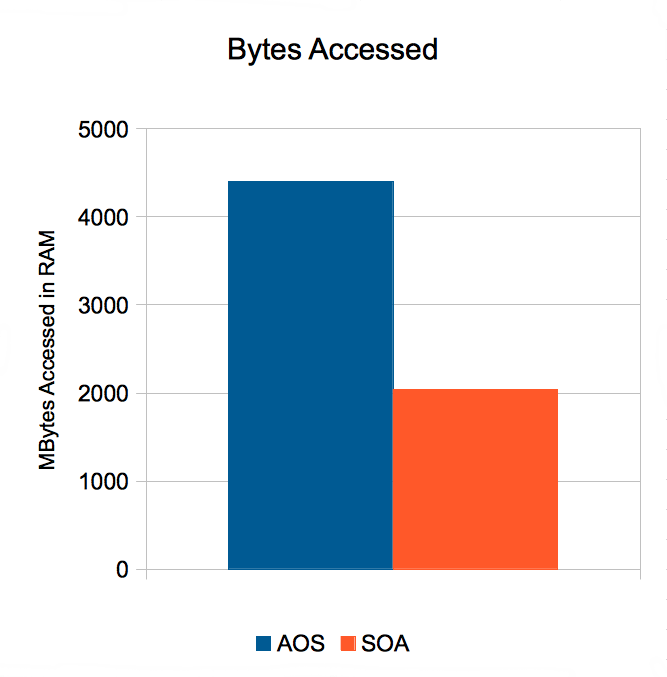
\includegraphics[width=\columnwidth]{images/report.april/bytes.png}
	\end{center}
	\caption{Comparison of number of bytes accessed by each version. Measured with the \texttt{BUS\_TRANS\_MEM} native hardware event (see \cref{sec:method,sec:events}).}
	\label{fig:bytes}
\end{figure}

\begin{figure}[!p]
	\begin{center}
		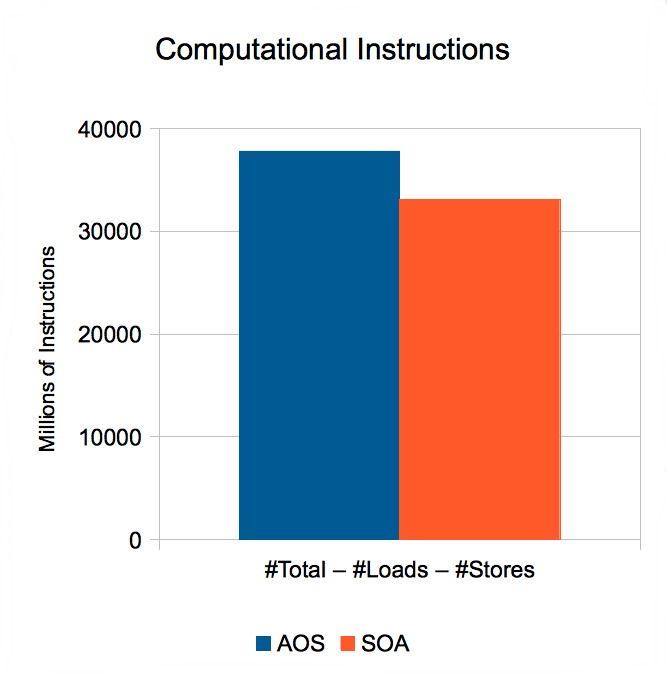
\includegraphics[width=\columnwidth]{images/report.april/instructions.png}
	\end{center}
	\caption{Comparison of computational instructions completed by each version (see \cref{sec:method}).}
	\label{fig:instructions}
\end{figure}

\begin{figure}[!p]
	\begin{center}
		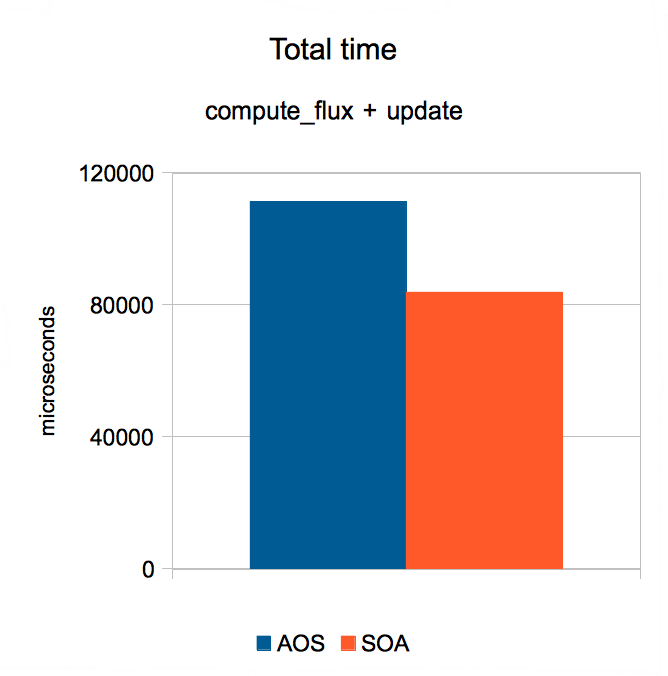
\includegraphics[width=\columnwidth]{images/report.april/time.png}
	\end{center}
	\caption{Comparison of execution time (only for the core functions) achieved by each version. Measured using the operative system timers, limited to the core functions, in a fully reserved SeARCH Group 201 node (see \cref{sec:method}).}
	\label{fig:time}
\end{figure}

\Cref{fig:bytes} shows the median values measured for the bytes accessed to RAM in each version. One can easily see the new version transfers less than half the bytes of the previous one. This improvement alone explains the doubled value for the computational intensity.

Regarding the number of instructions, \cref{fig:instructions} shows the SOA version in fact reduced the total number of computational instructions (by around 12\%). This implies that the algorithm will only attain more instructions per second if the execution time decreased by a greater factor. It also limits the influence of having less bytes being accessed in RAM in the computational intensity.

As expected, since the roofline shows only a slight increase in the number of attained instructions per second, \cref{fig:time} shows a decrease in the execution time by a factor around 24\%. Although the execution time decrease factor is the double of the instruction decrease factor, \Cref{eq:attainedfraction} proves the number of attained computational instructions (0.34 in AOS and 0.39 in SOA) increased by an expected factor related with these decreases.

\begin{IEEEeqnarray}{CrClC}
                & \mathrm{Attained\ instructions}/s & = & \frac{\#\mathrm{instructions}}{\Delta t} & \Leftrightarrow	\label{eq:attainedfraction}\\
\Leftrightarrow & f\left(\mathrm{Att.\ insts.}/s\right) & = & \frac{(1-0.12)\#\mathrm{insts.}}{(1-0.24)\Delta t} & \Leftrightarrow	\nonumber\\
\Leftrightarrow & f & = & \frac{0.88}{0.76} & \Leftrightarrow	\nonumber\\
\Leftrightarrow & f & = & 1.16 & \enspace .\nonumber
\end{IEEEeqnarray}

\begin{figure}[!htp]
	\begin{center}
		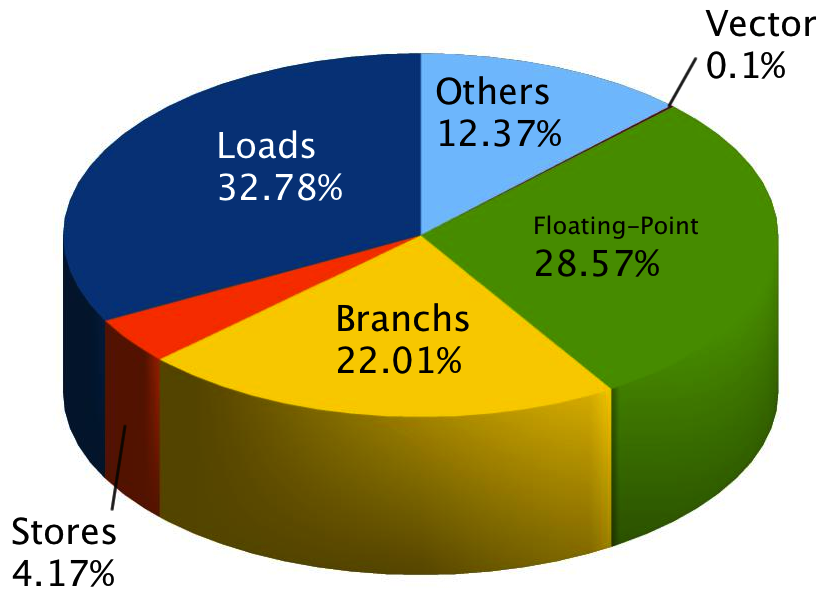
\includegraphics[width=\columnwidth]{images/report.april/instmxSOA.png}
	\end{center}
	\caption{Instruction mix for the new version (SOA).}
	\label{fig:instmxSOA}
\end{figure}

The decrease in the number of instructions (7\% for the total instructions completed) also allows to justify the new version's instruction mix. On the contrary of what was expected, the fraction of load instructions was not reduced, but instead it increased. The decrease in the total number of instructions was mostly due to the vector instructions (which are nearly null\footnote{With the right flags, \texttt{gcc} was able to increase considerably this fraction, reducing both the total of completed instructions and execution time, but only between 1\% and 2\%. Therefore, this option was not explored further.}) and the remaining non-specified instructions. This shows that although the program was improved (it was already stated that the execution time decreased), this did not happen due to a decrease in the required data, which implies the major improvement happened with cache management. In fact, \cref{fig:missrates} shows that despite having the same miss rate in the L1 cache, the SOA version decreased the miss rate in the L2 cache by almost 7\%.

\begin{figure}[!htp]
	\begin{center}
		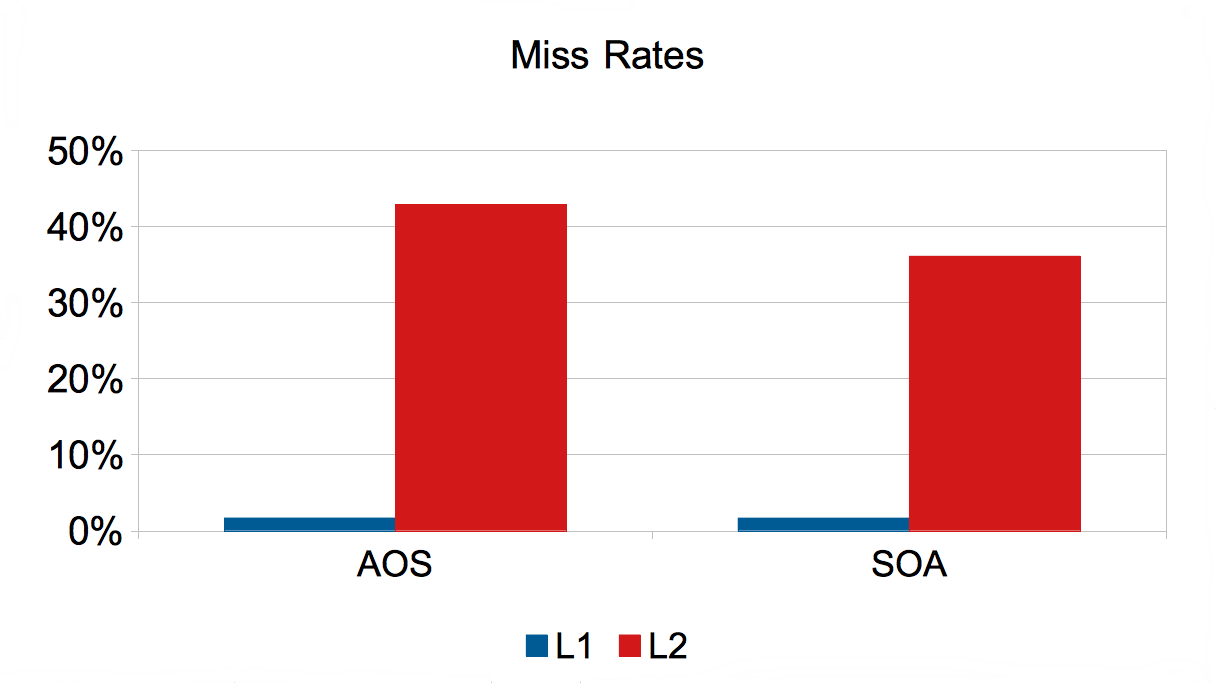
\includegraphics[width=\columnwidth]{images/report.april/missrates.png}
	\end{center}
	\caption{Comparison of the miss rates in each cache level for each version.}
	\label{fig:missrates}
\end{figure}

Parallelism granularity remains unchanged in the new version, as shows \cref{fig:steptimeSOA} (around 10 milliseconds for the fastest execution of \texttt{compute\_flux}). The same is true for the workload balance (see \cref{fig:tasktimeSOA}) -- the core functions have clearly different execution times, but equal workload between threads in the same function.

\begin{figure}[!p]
	\begin{center}
		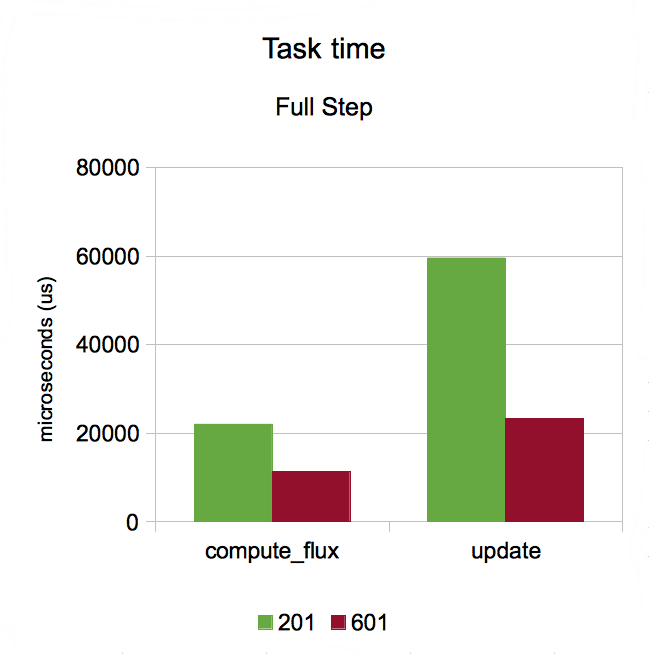
\includegraphics[width=\columnwidth]{images/report.april/steptimeSOA.png}
	\end{center}
	\caption{Median execution times for a full execution of each core function in each kind of computational node. Measured for the new version (SOA).}
	\label{fig:steptimeSOA}
\end{figure}

\begin{figure}[!p]
	\begin{center}
		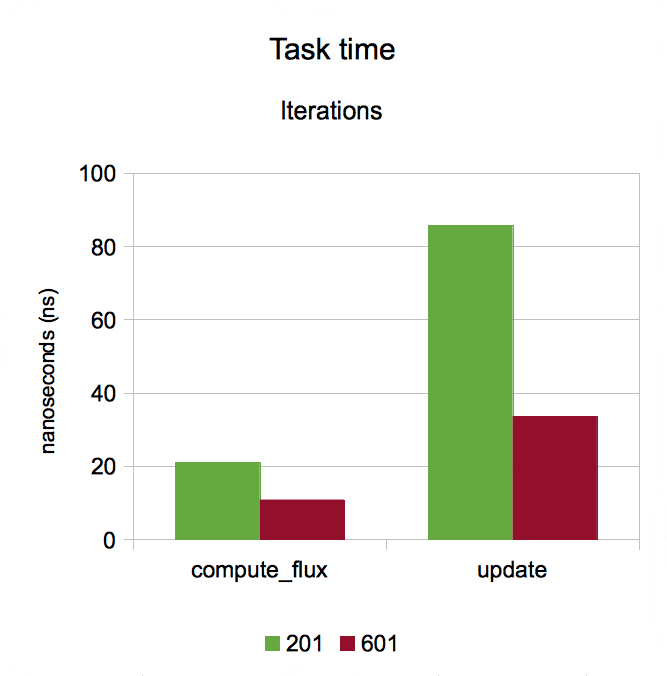
\includegraphics[width=\columnwidth]{images/report.april/tasktimeSOA.png}
	\end{center}
	\caption{Minimum execution times for a single iteration of the inner cycle of each core function in each kind of computational node. Measured for the new version (SOA).}
	\label{fig:tasktimeSOA}
\end{figure}

Lastly, focus is given to the speedups attained with each version. \Cref{fig:executiontime} shows that the new memory access pattern improved the sequential execution time by a factor greater than the previous version. Furthermore, \cref{fig:speedup} shows that by adding parallelization to this new version, the algorithm attained greater speedups compared to the respective sequential version than the previous version. The best execution times are attained with 4 threads in SeARCH Group 201 nodes and with 12 threads in SeARCH Group 601. To note that using the 24 threads available in SeARCH Group 601 (using the Intel\textregistered Hyper-Threading Technology), the execution time increases (almost as much as the sequential version).

\begin{figure*}[!p]
	\begin{center}
		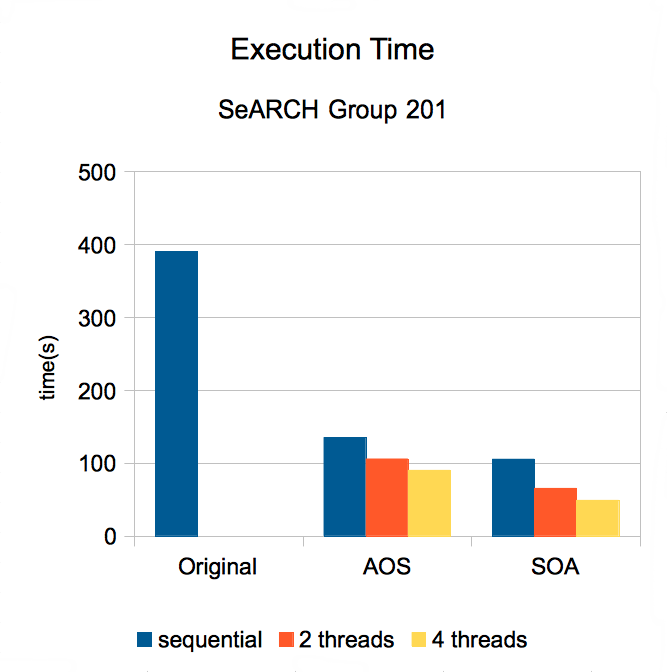
\includegraphics[width=\columnwidth]{images/report.april/time201.png}
		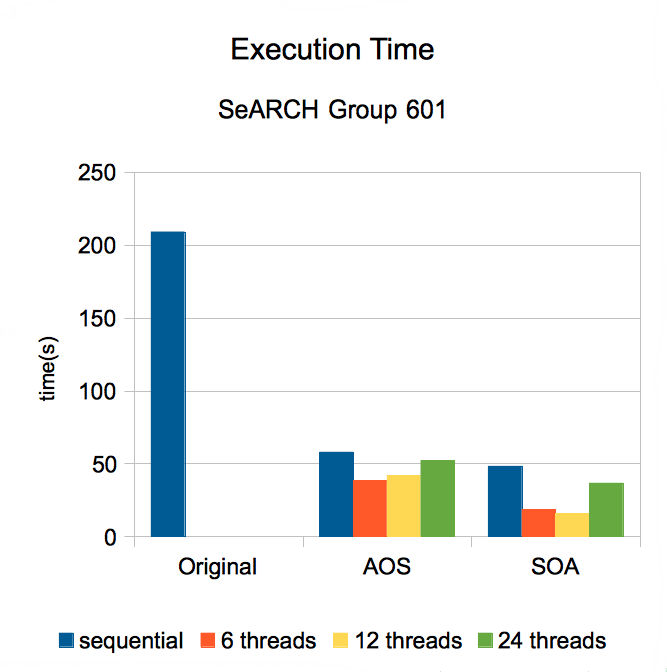
\includegraphics[width=\columnwidth]{images/report.april/time601.png}
		\caption[Execution Times]{Execution times for each version in each kind of computational node.}
		\label{fig:executiontime}
	\end{center}
\end{figure*}

\begin{figure*}[!p]
	\begin{center}
		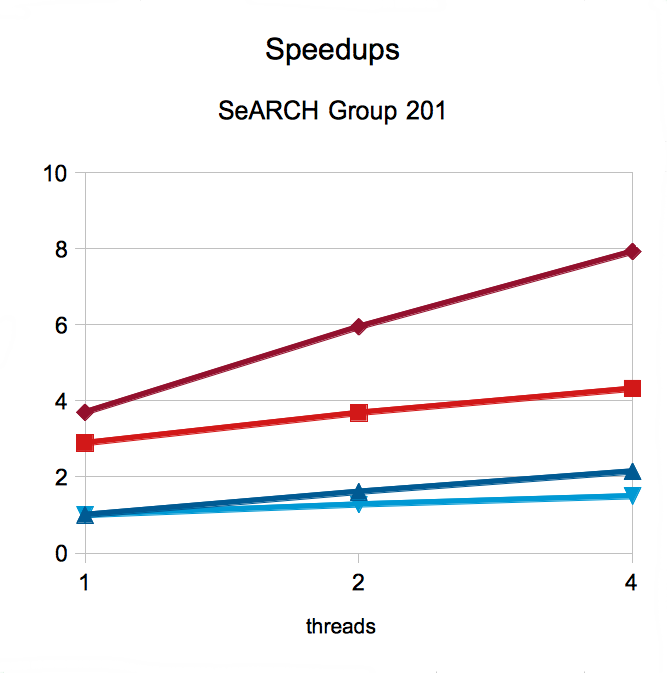
\includegraphics[width=\columnwidth]{images/report.april/speedup201.png}
		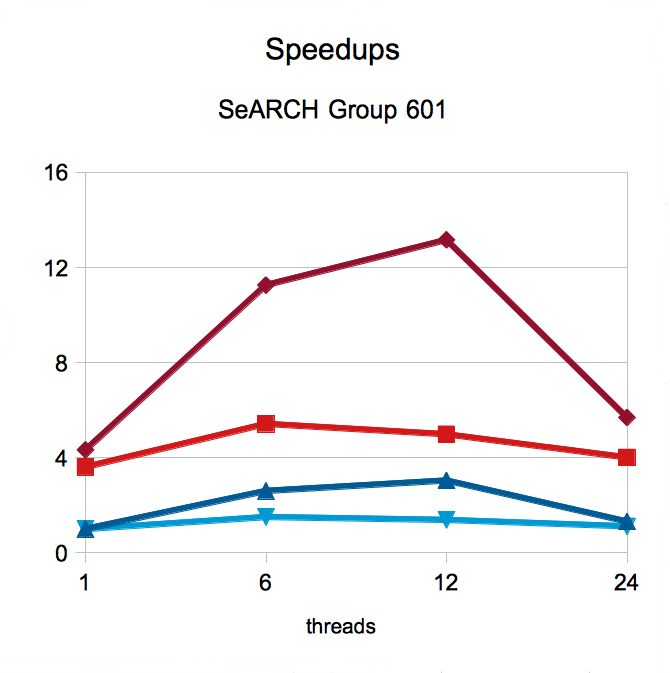
\includegraphics[width=\columnwidth]{images/report.april/speedup601.png}
		
\includegraphics[width=\columnwidth]{images/report.april/speedup-legend.png}
	\end{center}
	\caption[Speedups]{Speedups attained with each version in each kind of computational node. The red lines show the speedups of the two versions when compared to the original code. The blue lines show the speedups compared with each version's sequential code. Light colors represent the previous version (AOS). Dark colors represent the new version (SOA).}
	\label{fig:speedup}
\end{figure*}

In the previous report, the parallel code fraction was measured to be 94\%. \Cref{tab:speedupmax} shows the calculated values for the maximum speedup possible according to Amdahl's Law (see \cref{eq:amdahl}, where $N$ is the number of processors, $p$ is the parallel code fraction and $s = 1 - p$) and the effectively attained values (compared to the respective sequential version). The advantage of the new version is clear in these results, which demonstrate the improvement in the algorithm's scalability. Despite that, one may notice that for SeARCH Group 601 nodes, although the execution time is lower than in SeARCH Group 201 nodes, the speedup attained from adding parallelization is in fact lower. This is most probably because SeARCH Group 601 nodes have a NUMA architecture.

\begin{table}[!htp]
	\begin{center}
		\begin{tabular}{cccccc}
		\hline
		\textbf{Threads} & \textbf{Maximum} & \textbf{AOS} & & \textbf{SOA} &	\\
		\hline
		\hline
		 4 &  3.39 & 1.49 & 44\% & 2.14 & 63\%	\\
		\hline
		12 &  7.23 & 1.38 & 19\% & 3.04 & 42\%	\\
		\hline
		\end{tabular}
	\end{center}
	\caption{Comparison between maximum and attained speedup values for the best execution times (4 threads in SeARCH Group 201 nodes, and 12 threads in SeARCH Group 601 nodes). Maximum values calculated according to Amdahl's Law.}
	\label{tab:speedupmax}
\end{table}

\begin{IEEEeqnarray}{rCl}
\mathrm{speedup_{max}} & = & \frac{1}{s + \frac{p}{N}}	\enspace .\label{eq:amdahl}
\end{IEEEeqnarray}







\section{Conclusion}
\label{sec:conclusion}
Throughout this document, the previous code version of the \texttt{polu} program was analyzed and improved by changing the data structures and consequently the memory access pattern.

The analysis performed on the AOS version allowed to exclude parallelism granularity, excessive synchronization and task imbalance as causes for the poor locality of the algorithm. Furthermore, this analysis allowed a better understanding of the nearly chaotic memory access pattern throughout the entire execution, identifying flaws which could be easily changed with a different approach.

The previous code was improved with by changing the data structures from \textit{Arrays-of-Structures} to \textit{Structures-of-Arrays}, thus allowing the core functions to dismiss pieces of data not required for the computation. This change also favored the ordered iteration over the data collections which compose the domain.

Both versions were thoroughly measured in order to build a complete and accurate profile of their execution. A special emphasis was given to the change from operational intensity to computational (or arithmetic) intensity, which provides a more complete overview of the program's performance, given that the fraction of floating-point instructions is no more than a quarter.

The new version bested the previous implementation in every measure, from execution times to parallel speedups. High effort was made towards justifying the evolution in the computational intensity and the apparent apathy behind the number of attained instructions per second. The new code was proved to diminish the need to load data from RAM to less than half, decrease slightly the number of instructions and considerably reduce execution time, when compared to the AOS version.

The new SOA version presented higher speedup values, running more than 13 times faster than the original code (when using 12 threads). It also revealed better scalability values, especially if executed in an UMA architecture -- where it achieved more than half the limit calculated with Amdahl's Law.

As for future work regarding the improvement of locality for this algorithm in a shared memory environment, it is possible that Hoppe's work could be adapted to this case, optimizing the accesses to the mesh in the fashion as it optimizes the process of drawing 3D objects.

% GCC vs ICC
Another test that was considered interesting for this document was a comparative benchmark using a different compiler, specifically Intel\textsuperscript{\textregistered} C/C++ Compiler (ICC). The required changes to the compilation process were made, so that ICC was used instead of GCC, and different executables were generated successfully. These were submitted to the SeARCH Group 601 nodes. However, possibly due to configuration problems with ICC libraries in the said SeARCH nodes, most of the execution attempts were unsuccessful, with some exceptions.%. There were however some successful executions.

Both the GCC and the ICC versions were tested with OpenMP directives set to run with 6, 12 and 24 threads. For most of the cases, GCC was able to perform better (around 10\% less execution time in each case), with the exception of the cases with 24 threads. In this situation the program tries to take advantage of the Intel\textsuperscript{\textregistered} Hyper-Threading Technology, since there are two threads allocated to each physical core. Since this cases were performed better by ICC, it shows that the Intel\textsuperscript{\textregistered} compiler generates code that deals better with Hyper-Threading. This difference, however, was not significant, and the overall execution was actually slower than the 12 threads version, due to obvious memory limitations, hindering the execution of such large amount of threads. Further investigation also suggested that different, less obvious optimization flags may provide better results.

Finally, problems using the Intel\textsuperscript{\textregistered} Compiler (either from configuration problems or from lack of experience) prevented more accurate and complete results on this subject.
% what was done and found
%\subsection{Future Work}
% what can be done next

\bibliographystyle{IEEE}
\bibliography{report.april}

\appendix
\section{Environmental Setup}
\label{sec:environment}
% characteristics of the experimental environment
Two different types of nodes from the SeARCH cluster\footnote{\url{http://search.di.uminho.pt}} were used for the required measurements.

The nodes of the first type, referred to in this document as SeARCH Group 201, have two dual-core processors with a clock frequency of 2.0 GHz and 4 GB of RAM (see \cref{tab:group201} for further detail regarding hardware). The specially allocated node 201-1, accessible only by exclusive SSH login (which prevents the occurrence of interference), was used to conduct the detailed profiling through the PAPI library. This group was used to perform scalability tests up to 4 threads, each test being performed in a single fully reserved node.

The second type -- SeARCH Group 601 -- contains nodes which have two hex-core processors (with Intel\textregistered Hyper-Threading Technology) and 12 GB of RAM (see \cref{tab:group601} for further detail regarding hardware). This group was used to perform scalability tests up to 24 threads, each test being performed in a single fully reserved node.

\begin{table}[!htp]
	\begin{tabular}{ll}
		\hline
		Processors per node: & 2	\\
		Processor model: & Intel\textregistered Xeon\textregistered E5130\\
		Cores per processor: & 2	\\
		Threads per core: & 1	\\
		Clock frequency: & 2.00 GHz	\\
		\hline
		L1 cache: & 32 KB + 32 KB per core	\\
		L2 cache: & 4 MB shared	\\
		L3 cache: & N/A	\\
		RAM: & 4 GB	\\
		\hline
	\end{tabular}
	\caption[SeARCH Group 201 hardware description]{SeARCH Group 201 hardware description. See \cite{xeon5100} for further detail about this processor.}
	\label{tab:group201}
\end{table}
\begin{table}[!htp]
	\begin{tabular}{ll}
		\hline
		Processors per node: & 2	\\
		Processor model: & Intel\textregistered Xeon\textregistered X5650\\
		Cores per processor: & 6	\\
		Threads per core: & 2	\\
		Clock frequency: & 2.66 GHz	\\
		\hline
		L1 cache: & 32 KB + 32 KB per core	\\
		L2 cache: & 256 KB per core	\\
		L3 cache: & 12 MB shared	\\
		RAM: & 12 GB	\\
		\hline
	\end{tabular}
	\caption[SeARCH Group 601 hardware description]{SeARCH Group 601 hardware description. See \cite{xeon5600} for further detail about this processor.}
	\label{tab:group601}
\end{table}


\section{Methodology}
\label{sec:method}
% which experiments were performed
Two different kinds of measurements are performed with each version mentioned in this document. 

The first uses the operating system timers to measure total and partial execution time -- focus is given to the execution time of the whole program and to each of the core functions. The measurements are performed using a custom object-oriented interface, optimized as very short inline definitions to minimize the measurement overhead to the bare minimum.

The second kind uses the PAPI library, which allows the usage of hardware counters to obtain detailed information about the program's execution. To be more specific, these measurements are limited only to the core executions, since these will be the targets of parallelization. Since a correct usage of this library requires some repetitive code (as testing if the functions were successful), an object-oriented wrapper was designed to automatically deal with such issues. In addition, the abstraction provided by this wrapper allowed an easier management of the code to profile, given the many events measured.

The following measurements were performed to retrieve the results mentioned throughout this document:
\begin{description}
	\item[Computational Intensity]{Ratio between the number of computational instructions completed and the number of bytes accessed in RAM. This is used to build the rooflines, namely to provide the data needed to plot the program in the correct way. Every instruction except for loads and stores are considered computational instructions. This measurement includes the \texttt{BUS\_TRANS\_MEM}, \texttt{PAPI\_LD\_INS}, \texttt{PAPI\_SR\_INS} and \texttt{PAPI\_TOT\_INS} hardware events from the PAPI library. The execution time considered to calculate the attained number of instructions per second includes only the core functions execution since this is the scope used with the PAPI library.
	
	In the previous report the roofline was built using operational intensity (ratio between floating-point operations and bytes accessed). Yet this measure does not take into consideration the other kinds of instructions completed during execution, such as branches. The instruction mix measured in \cref{sec:aos} proves that such measure is unfit for this case, and that computational intensity is a much more complete approach.
	}
	\item[Instruction Mix]{Used to identify the fraction of instructions related with computation and with memory accesses and to identify the influence of branches. Includes the \texttt{PAPI\_BR\_INS}, \texttt{PAPI\_FP\_INS}, \texttt{PAPI\_LD\_INS}, \texttt{PAPI\_SR\_INS}, \texttt{PAPI\_TOT\_INS} and \texttt{PAPI\_VEC\_INS} preset hardware events from the PAPI library.
	}
	\item[Step \& Task time]{These are used to evaluate the parallelism granularity and the work balance.
	
	Step time refers to the time needed to completely execute one of the core functions (a step or phase of the algorithm). It is measured using the operative system timers, limited to the target function. Since the parallel zone in each function includes the entire code, a proper granularity would require the minimum execution time of the function to be significantly greater than the overhead of creating the parallel zone.
	
	Task time refers to the time required to execute only one iteration of the inner cycle of each core function. This allows to estimate the workload performed by each function by comparing the execution time of a single iteration. Note that, as explained in \cref{sec:aos}, there is no imbalance between different threads inside any of the core functions, and therefore it is not required to measure the variance of executing a single iteration for any function.
	}
	\item[Miss Rates]{Used to analyze the locality of each version. Includes the \texttt{PAPI\_L1\_TCA}, \texttt{PAPI\_L1\_TCM}, \texttt{PAPI\_L2\_TCA} and \texttt{PAPI\_L2\_TCM} preset hardware events from the PAPI library.
	}
\end{description}

The value considered for each measurement is the median of the values for at least 10 different executions. When nothing is mentioned, a value should be assumed to be the median. Measurements such as task time use the minimum measured -- such cases are explicitly identified either in the graph or table describing the results.

\section{PAPI Events}
\label{sec:events}
This section is meant to provide explanation about the goal of each of the events used with the PAPI library:
\begin{description}
	\item[\ttfamily BUS\_TRANS\_MEM]{(Native event) Number of transactions in the bus connecting the processor to the memory -- this is considered to retrieve the number of accesses to RAM;}
	\item[\ttfamily PAPI\_BR\_INS]{(Preset event) Number of branch instructions completed;}
	\item[\ttfamily PAPI\_FP\_INS]{(Preset event) Number of floating-point instructions completed;}
	\item[\ttfamily PAPI\_L1\_TCA]{(Preset event) Total cache accesses in the L1 cache;}
	\item[\ttfamily PAPI\_L1\_TCM]{(Preset event) Total cache misses in the L1 cache;}
	\item[\ttfamily PAPI\_L2\_TCA]{(Preset event) Total cache accesses in the L2 cache;}
	\item[\ttfamily PAPI\_L2\_TCM]{(Preset event) Total cache misses in the L2 cache;}
	\item[\ttfamily PAPI\_LD\_INS]{(Preset event) Number of load instructions completed;}
	\item[\ttfamily PAPI\_SR\_INS]{(Preset event) Number of store instructions completed;}
	\item[\ttfamily PAPI\_TOT\_INS]{(Preset event) Total number of instructions completed;}
	\item[\ttfamily PAPI\_VEC\_INS]{(Preset event) Number of vector instructions completed.}
\end{description}

\section{Roofline Model}
\label{sec:roofline}
%explains how the roofline was built
The roofline models used throughout this document were prepared according to the guidelines in \cite{williams08}, except for the memory bandwidth roof.

As stated before in \cref{sec:aos:results,sec:method}, computational intensity (or arithmetic intensity) is a more complete measure for the program studied in this document. Also, as mentioned in \cref{sec:method}, only a particular node belonging to SeARCH Group 201 was used to perform the detailed profiling. Therefore, only one roofline model is required to reflect the hardware limitations of such computational nodes.

According to \cite{xeon5100,intelsys,inteloptimize}, these nodes' micro architecture is Intel\textregistered Core\texttrademark, which is capable of decoding up to five instructions per cycle, has a throughput of up to 4 instructions per cycle and three full arithmetic logical units, where each has a throughput of one instruction per cycle for many kinds of computational instructions. This binds the peak throughput of computational instructions at 3 per cycle.

Since each core has a peak throughput of 3 computational instructions per cycle, each processor has 2 cores at a clock frequency of 2.0 GHz, and each node has 2 processors, this results in a peak of
\begin{IEEEeqnarray}{rCl}
3\times 2\times 2\times 10^{9}\times 2 & = & 24\;\mathrm{GInstructions/s}\enspace .
\end{IEEEeqnarray}
This value corresponds to the CPU roof.

Although \cite{williams08} recommends using ``a series of highly tuned versions of the STREAM benchmark'', the creation of such versions is out of the scope of this project. As such, the peak memory bandwidth was measured running the original STREAM benchmark in a SeARCH Group 201 node. The benchmark returned a peak value of 4.78 GB/s, which is the memory roof.

As for CPU ceilings, these were calculated decreasing the number of cores used, first by using only one processor (half the peak), then by removing thread-level parallelism (one core, a quarter of the peak). As measured in the previous report, this algorithm already presents itself with a high balance of floating-point multiplications and additions (two thirds of the TLP ceiling, as one of the ALUs would remain idle). The last CPU ceiling remaining would mean removing all the instruction-level parallelism (half the Mul/Add balance ceiling, only one ALU active).

Lastly, the absence of dual channel was used as the only memory ceiling. The influence of any other mechanism such as prefetch or unit stride accesses would have to be properly measured with the recommended tuned versions, which are not available for this document.

\Cref{fig:roofline} shows the resulting roofline model for the nodes of SeARCH Group 201.

\begin{figure}[!htp]
	\begin{center}
		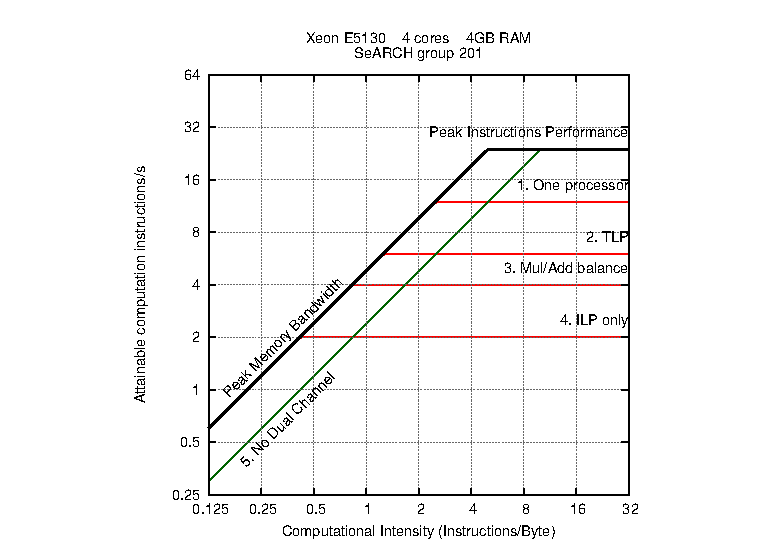
\includegraphics[width=\columnwidth]{images/report.april/roofline.eps}
	\end{center}
	\caption{Roofline for SeARCH Group 201.}
	\label{fig:roofline}
\end{figure}

\end{document}
